% -------------- TABLA PARA REQUERIMIENTOS FUNCIONALES ---------------- %
% Nomenclatura para la prioridad:
%	MA - Muy Alta
%	A - Alta
%	M - Media
%	B - Baja
%	MB - Muy Baja

\begin{table}[htbp!]
    \begin{requerimientos}

%-----------------------------------------------------Requerimeintos de Usuario-----------------------------------------------------------

        \FRitem{SP4-U1}{Registrar Programa Académico}{El usuario Jefe de Innovación Educativa registra los datos del Programas Académicos, acorde a la entidad Programa Académico del \hyperref[MDD]{Modelo de Datos}.}{A}{Origen}
        \label{SP4-U1}

        \FRitem{SP4-U2}{Registrar Plan de Estudios}{El usuario Jefe de Innovación Educativa registra los datos del Plan de estudios , acorde a la entidad Plan de Estudios del \hyperref[MDD]{Modelo de Datos}.}{A}{Origen}
        \label{SP4-U2}

        \FRitem{SP4-U3}{Registrar Unidad de Aprendizaje}{El usuario Docente registra los datos de las Unidades de Aprendizaje, de acorde a la entidad Unidad de Aprendizaje del \hyperref[MDD]{Modelo de Datos},  que contiene el Mapa Curricular.}{A}{Origen}
        \label{SP4-U3}

        \FRitem{SP4-U4}{Registrar Usuarios}{El usuario Jefe de Innovación Educativa registra a los usuarios (Analista y Docente).}{A}{Origen}
        \label{SP4-U4}

        \FRitem{SP4-U5}{Consultar Programas Académicos }{El usuario Jefe de Innovación Educativa visualiza la informacion de los Programas Académicos.}{A}{Origen}
        \label{SP4-U5}

        \FRitem{SP4-U6}{Consultar Planes de Estudios }{El usuario Jefe de Innovación Educativa visualiza la informacion de los Planes de Estudios.}{A}{Origen}
        \label{SP4-U6}

        \FRitem{SP4-U7}{Consultar Tareas}{El usuario consulta las tareas en las que esta asignado.}{A}{Origen}
        \label{SP4-U7}

        \FRitem{SP4-U8}{Consultar Mapa Curricular }{El usuario Docente visualiza la totalidad de los contenidos del Mapa Curricular registrados.}{A}{Origen}
        \label{SP4-U8}

        \FRitem{SP4-U9}{Consultar Usuarios}{El usuario  Jefe de Innovación Educativa consulta los usuarios.}{A}{Origen}
        \label{SP4-U9}

        \FRitem{SP4-U10}{Finalizar Carga Mapa Curricular}{El usuario Docente finaliza el registro de todas las Unidades de Aprendizaje que contiene el Mapa  Curricular.}{A}{Origen}
        \label{SP4-U10}

        \FRitem{SP4-U11}{Asignar tareas a los usuarios de la Unidad Académica}{El usuario Jefe de Innovación Educativa asigna tareas a los usuarios.}{A}{Origen}
        \label{SP4-U11}

        \FRitem{SP4-U12}{Generar Tareas}{El usuario Jefe de Innovación Educativa genera las tareas de registro (Mapas Curriculares y Programas Sintéticos).}{A}{Origen}
        \label{SP4-U12}

    \end{requerimientos}
\caption{Requerimientos de Usuario 1/2 del subproceso de elaboración del Mapa Curricular}
\label{tbl:SP4-RU1}
\end{table}

\begin{table}[htbp!]
    \begin{requerimientos}
        \FRitem{SP4-U13}{Consultar Tareas}{Los usuarios visualizan las tareas a las que están asignados.}{A}{Origen}
        \label{SP4-U13}

        \FRitem{SP4-U14}{Enviar Comentarios}{ Los usuarios del Departamento de Innovación Educativa envían comentarios de corrección sobre el Mapa Curricular una vez que el registro haya finalizado.}{A}{Origen}
        \label{SP4-U14}

        \FRitem{SP4-U15}{Visualizar Comentarios}{ El Usuario Docente visualiza los comentarios hechos al Mapa Curricular, tanto por el Departamento de Innovación Educativa como por la DES.}{A}{Origen}
        \label{SP4-U15}

        \FRitem{SP4-U16}{Modificar Unidad de Aprendizaje}{El usuario Docente modifica los datos de las Unidades de Aprendizaje registradas.}{M}{Origen}
        \label{SP4-U16}

        \FRitem{SP4-U17}{Eliminar Unidad de Aprendizaje}{El usuario Docente elimina las Unidades de Aprendizaje registradas.}{M}{Origen}
        \label{SP4-U17}

        \FRitem{SP4-U18}{Guardar Avances del Mapa Curricular}{El usuario Docente guarda las Unidades de Aprendizaje que este vaya registrando.}{M}{Origen}
        \label{SP4-U18}

        \FRitem{SP4-U19}{Aprobar Mapa Curricular}{El usuario Jefe  de Innovación Educativa aprueba el Mapa Curricular una vez que el registro haya finalizado.}{M}{Origen}
        \label{SP4-U19}

        \FRitem{SP4-U20}{Revisar Mapa Curricular}{El usuario Analista revisa el Mapa Curricular una vez que el registro haya finalizado.}{B}{Origen}
        \label{SP4-U20}

        \FRitem{SP4-U21}{Modificar Programa Académico}{El usuario Jefe de Innovación Educativa modifica los datos de los Programas Académicos.}{B}{Origen}
        \label{SP4-U21}

        \FRitem{SP4-U22}{Modificar Plan de Estudios}{El usuario Jefe de Innovación Educativa modifica los datos del Plan de Estudios.}{B}{Origen}
        \label{SP4-U22}

        \FRitem{SP4-U23}{Modificar Información de Usuarios}{El usuario Jefe de Innovación Educativa modifica la información general de los usuarios.}{B}{Origen}
        \label{SP4-U23}

        \FRitem{SP4-U24}{Eliminar Usuarios}{El usuario Jefe de Innovación Educativa elimina a cualquier usuario.}{B}{Origen}
        \label{SP4-U24}

        \FRitem{SP4-U25}{Login}{El usuario ingresa a su cuenta.}{B}{Origen}
        \label{SP4-U25}

    \end{requerimientos}
\caption{Requerimientos  de Usuario 2/2 del subproceso de elaboración del Mapa Curricular}
\label{tbl:SP4-RU2}
\end{table}
%------------------------------------------------------Requerimeintos Funcionales-----------------------------------------------------------

\begin{table}[htbp!]
    \begin{requerimientos}

        \FRitem{SP4-F1}{Registrar Programa Académico}{El sistema debe permitir que el usuario de tipo "Jefe de Innovación Educativa" registre los datos de los Programas Académicos, acorde a la entidad Programa Académico del \hyperref[MDD]{Modelo de Datos}.}{A}{Origen}
        \label{SP4-F1}

        \FRitem{SP4-F2}{Registrar Plan de Estudios}{El sistema debe permitir que el usuario de tipo "Jefe de Innovación Educativa" registre los datos del Plan de estudios , acorde a la entidad Plan de Estudios del \hyperref[MDD]{Modelo de Datos}.}{A}{Origen}
        \label{SP4-F2}

        \FRitem{SP4-F3}{Registrar Unidad de Aprendizaje}{El sistema debe permitir que el usuario de tipo "Docente" registre los datos de las Unidades de Aprendizaje, acorde a la entidad Unidad de Aprendizaje del \hyperref[MDD]{Modelo de Datos}.}{A}{Origen}
        \label{SP4-F3}

        \FRitem{SP4-F4}{Registrar Usuarios}{El sistema debe permitir que el usuario de tipo "Jefe de Innovación Educativa" registre a los usuarios (Analista y Docente).}{A}{Origen}
        \label{SP4-F4}

        \FRitem{SP4-F5}{Consultar Programas Académicos }{El sistema debe permitir que el usuario de tipo "Jefe de Innovación Educativa" consulte los Programas Académicos.}{A}{Origen}
        \label{SP4-F5}

        \FRitem{SP4-F6}{Consultar Planes de Estudios }{El sistema debe permitir que el usuario de tipo "Jefe de Innovación Educativa" consulte los Planes de Estudios de los Programas Académicos.}{A}{Origen}
        \label{SP4-F6}

        \FRitem{SP4-F7}{Consultar Mapa Curricular }{El sistema debe permitir que el usuario de tipo "Docente" visualice todos los registros existentes del Mapa curricular.}{A}{Origen}
        \label{SP4-F7}

        \FRitem{SP4-F8}{Consultar Usuarios}{El sistema debe permitir que el usuario de tipo "Jefe de Innovación Educativa" consulte los usuarios.}{A}{Origen}
        \label{SP4-F8}

        \FRitem{SP4-F9}{Finalizar Tarea}{El sistema debe permitir que los usuarios indiquen cuando hayan finalizado una Tarea.}{A}{Origen}
        \label{SP4-F9}

        \FRitem{SP4-F10}{Asignar tareas a los usuarios de la Unidad Académica}{El sistema debe permitir que el usuario de tipo "Jefe de Innovación Educativa" asigne tareas a los usuarios.}{A}{Origen}
        \label{SP4-F10}

        \FRitem{SP4-F11}{Generar Tareas}{El sistema debe permitir que el usuario de tipo "Jefe de Innovación Educativa" genere las tareas de registro (Mapas Curriculares y Programas Sintéticos).}{A}{Origen}
        \label{SP4-F11}

        \FRitem{SP4-F120}{Consultar Tareas}{El sistema debe permitir que los usuarios visualicen las tareas a las que están asignados.}{A}{Origen}
        \label{SP4-F12}

        \FRitem{SP4-F13}{Validar congruencia en el Mapa Curricular}{ Si algunos de los datos ingresados se contradicen el sistema no permitirá que se guarden hasta resolver el conflicto.}{A}{Origen}
        \label{SP4-F13}

    \end{requerimientos}
    \caption{Requerimientos Funcionales 1/2 del subproceso de elaboración del Mapa Curricular}
    \label{tbl:SP4-RF1}
\end{table}

\begin{table}[htbp!]
    \begin{requerimientos}

        \FRitem{SP4-F14}{Enviar Comentarios}{ El sistema debe permitir que los usuarios de tipo "Analista" y  "Jefe de Innovación Educativa" envíen comentarios de corrección sobre el Mapa Curricular una vez que el usuario de tipo "Docente" haya finalizado el registro.}{A}{Origen}
        \label{SP4-F14}

        \FRitem{SP4-F15}{Visualizar Comentarios}{ El sistema debe permitir que el usuario de tipo "Docente" visualice los comentarios hechos a las tareas que este asignado, tanto los hechos por el Departamento de Innovación Educativa como por la DES.}{A}{Origen}
        \label{SP4-F15}

        \FRitem{SP4-F16}{Modificar Unidad de Aprendizaje}{El sistema debe permitir que el usuario de tipo "Docente" modifique lod dato de las Unidades de Aprendizaje que contiene el Mapa Curricular.}{M}{Origen}
        \label{SP4-F16}

        \FRitem{SP4-F17}{Eliminar Unidad de Aprendizaje}{El sistema debe permitir que el usuario de tipo "Docente" elimine las Unidades de Aprendizaje registradas.}{M}{Origen}
        \label{SP4-F17}

        \FRitem{SP4-F18}{Guardar Avances del Mapa Curricular}{El sistema debe permitirle al usuario Docente guardar las Unidades de Aprendizaje que éste vaya registrando.}{M}{Origen}
        \label{SP4-F18}

        \FRitem{SP4-F19}{Aprobar Mapa Curricular}{El sistema debe permitir que el usuario de tipo "Jefe de Innovación Educativa" apruebe el Mapa Curricular una vez que el usuario de tipo "Analista" haya finalizada la revisión.}{M}{Origen}
        \label{SP4-F19}

        \FRitem{SP4-F20}{Revisar Mapa Curricular}{El sistema debe permitir que el usuario de tipo "Analista" revise el Mapa Curricular  una vez que el usuario de tipo "Docente" haya finalizada el registro.}{B}{Origen}
        \label{SP4-F20}

        \FRitem{SP4-F21}{Modificar Programa Académico}{El sistema debe permitir que el usuario de tipo "Jefe de Innovación Educativa" modifique los datos de los Programas Académicos.}{B}{Origen}
        \label{SP4-F21}

        \FRitem{SP4-F22}{Modificar Plan de Estudios}{El sistema debe permitir que el usuario de tipo "Jefe de Innovación Educativa" modifique los datos del Plan de Estudios.}{B}{Origen}
        \label{SP4-F22}

        \FRitem{SP4-F23}{Modificar Usuarios de la Unidad Académica}{El sistema debe permitir que el usuario de tipo "Jefe de Innovación Educativa" modifique la información general de cualquier usuario.}{B}{Origen}
        \label{SP4-F23}

        \FRitem{SP4-F24}{Eliminar Usuarios de la Unidad Académica}{El sistema debe permitir que el usuario de tipo "Jefe de Innovación Educativa" elimine a cualquier usuario.}{B}{Origen}
        \label{SP4-F24}

        \FRitem{SP4-F25}{Notificar al Usuario}{El sistema informará al usuario de los cambios de estatus de las tareas a las que está asignado.}{B}{Origen}
        \label{SP4-F25}

        \FRitem{SP4-F26}{Login}{El sistema permitira al usuario ingresar a su cuenta.}{B}{Origen}
        \label{SP4-F26}

    \end{requerimientos}
    \caption{Requerimientos Funcionale 2/2 del subproceso de elaboración del Mapa Curricular}
    \label{tbl:SP4-RF2}
\end{table}

\begin{figure}[htbp]
    \begin{center}
        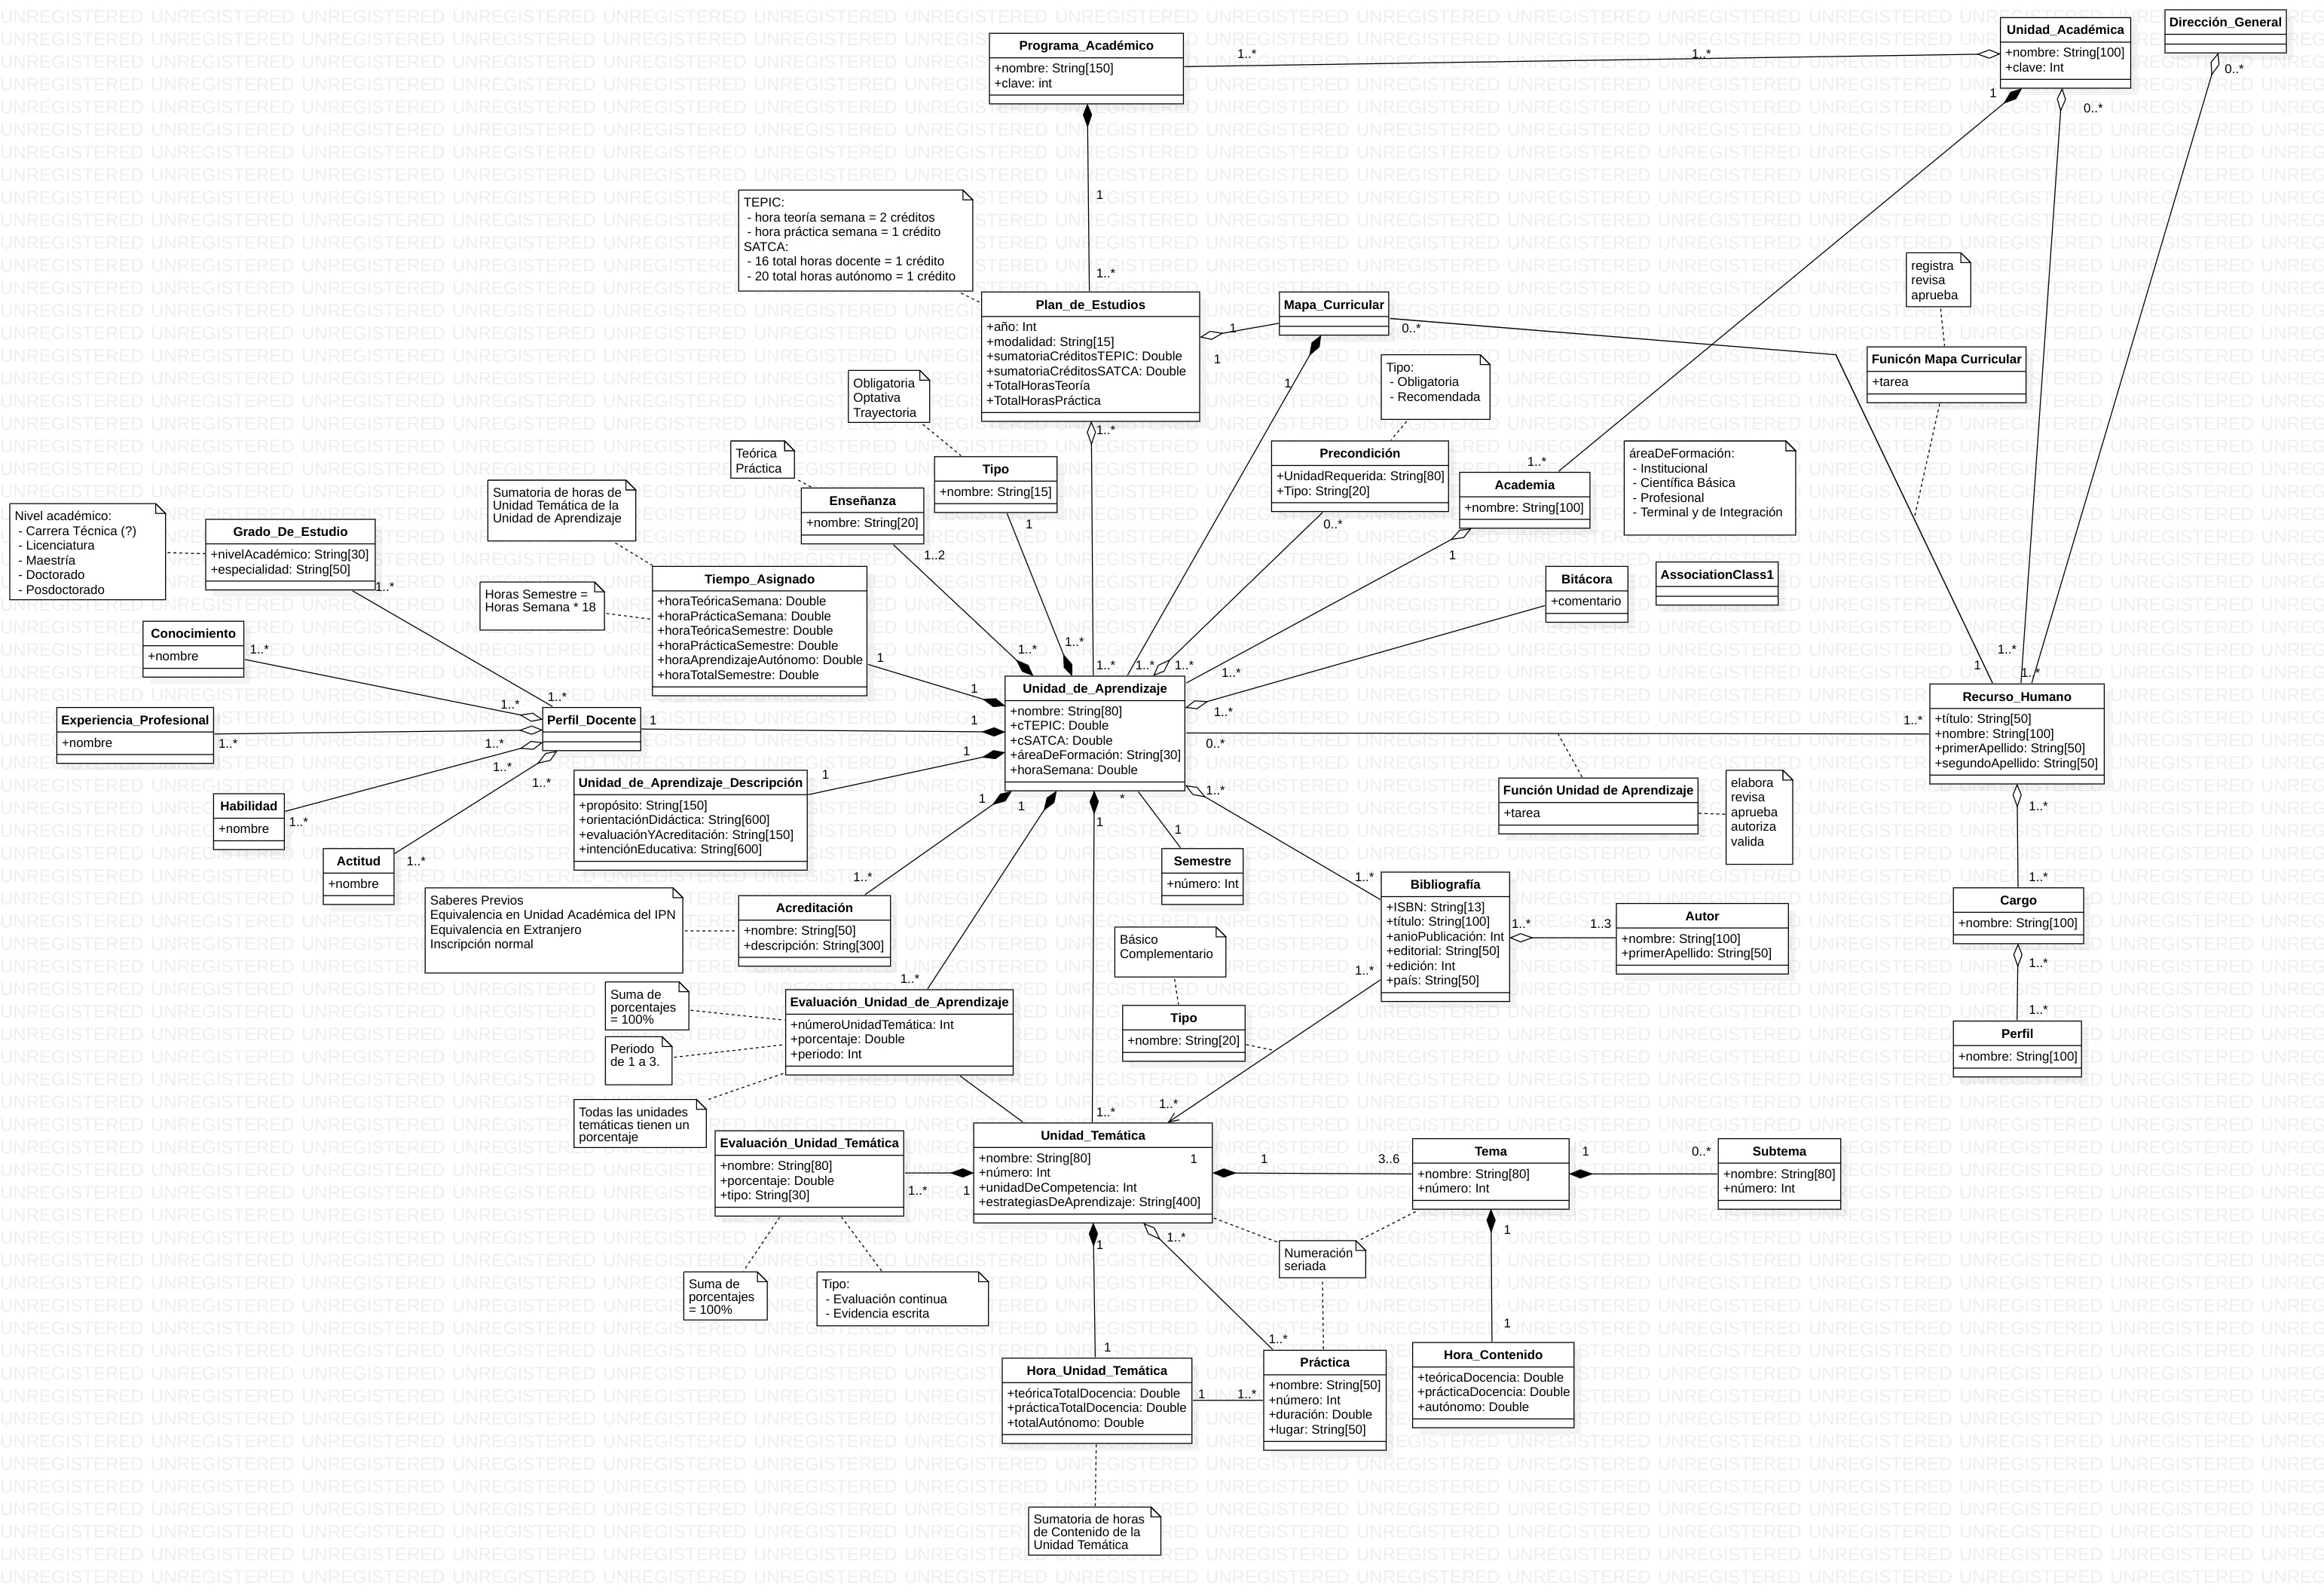
\includegraphics[width=.95\textwidth]{C2-DR/SP4/Image/ModeloDeDatosjpg}
        \label{MDD}
        \caption{Modelo de Datos Subproceso para la  Carga del Mapa Curricular}
    \end{center}
\end{figure}

\begin{figure}[htbp]
	\begin{center}
		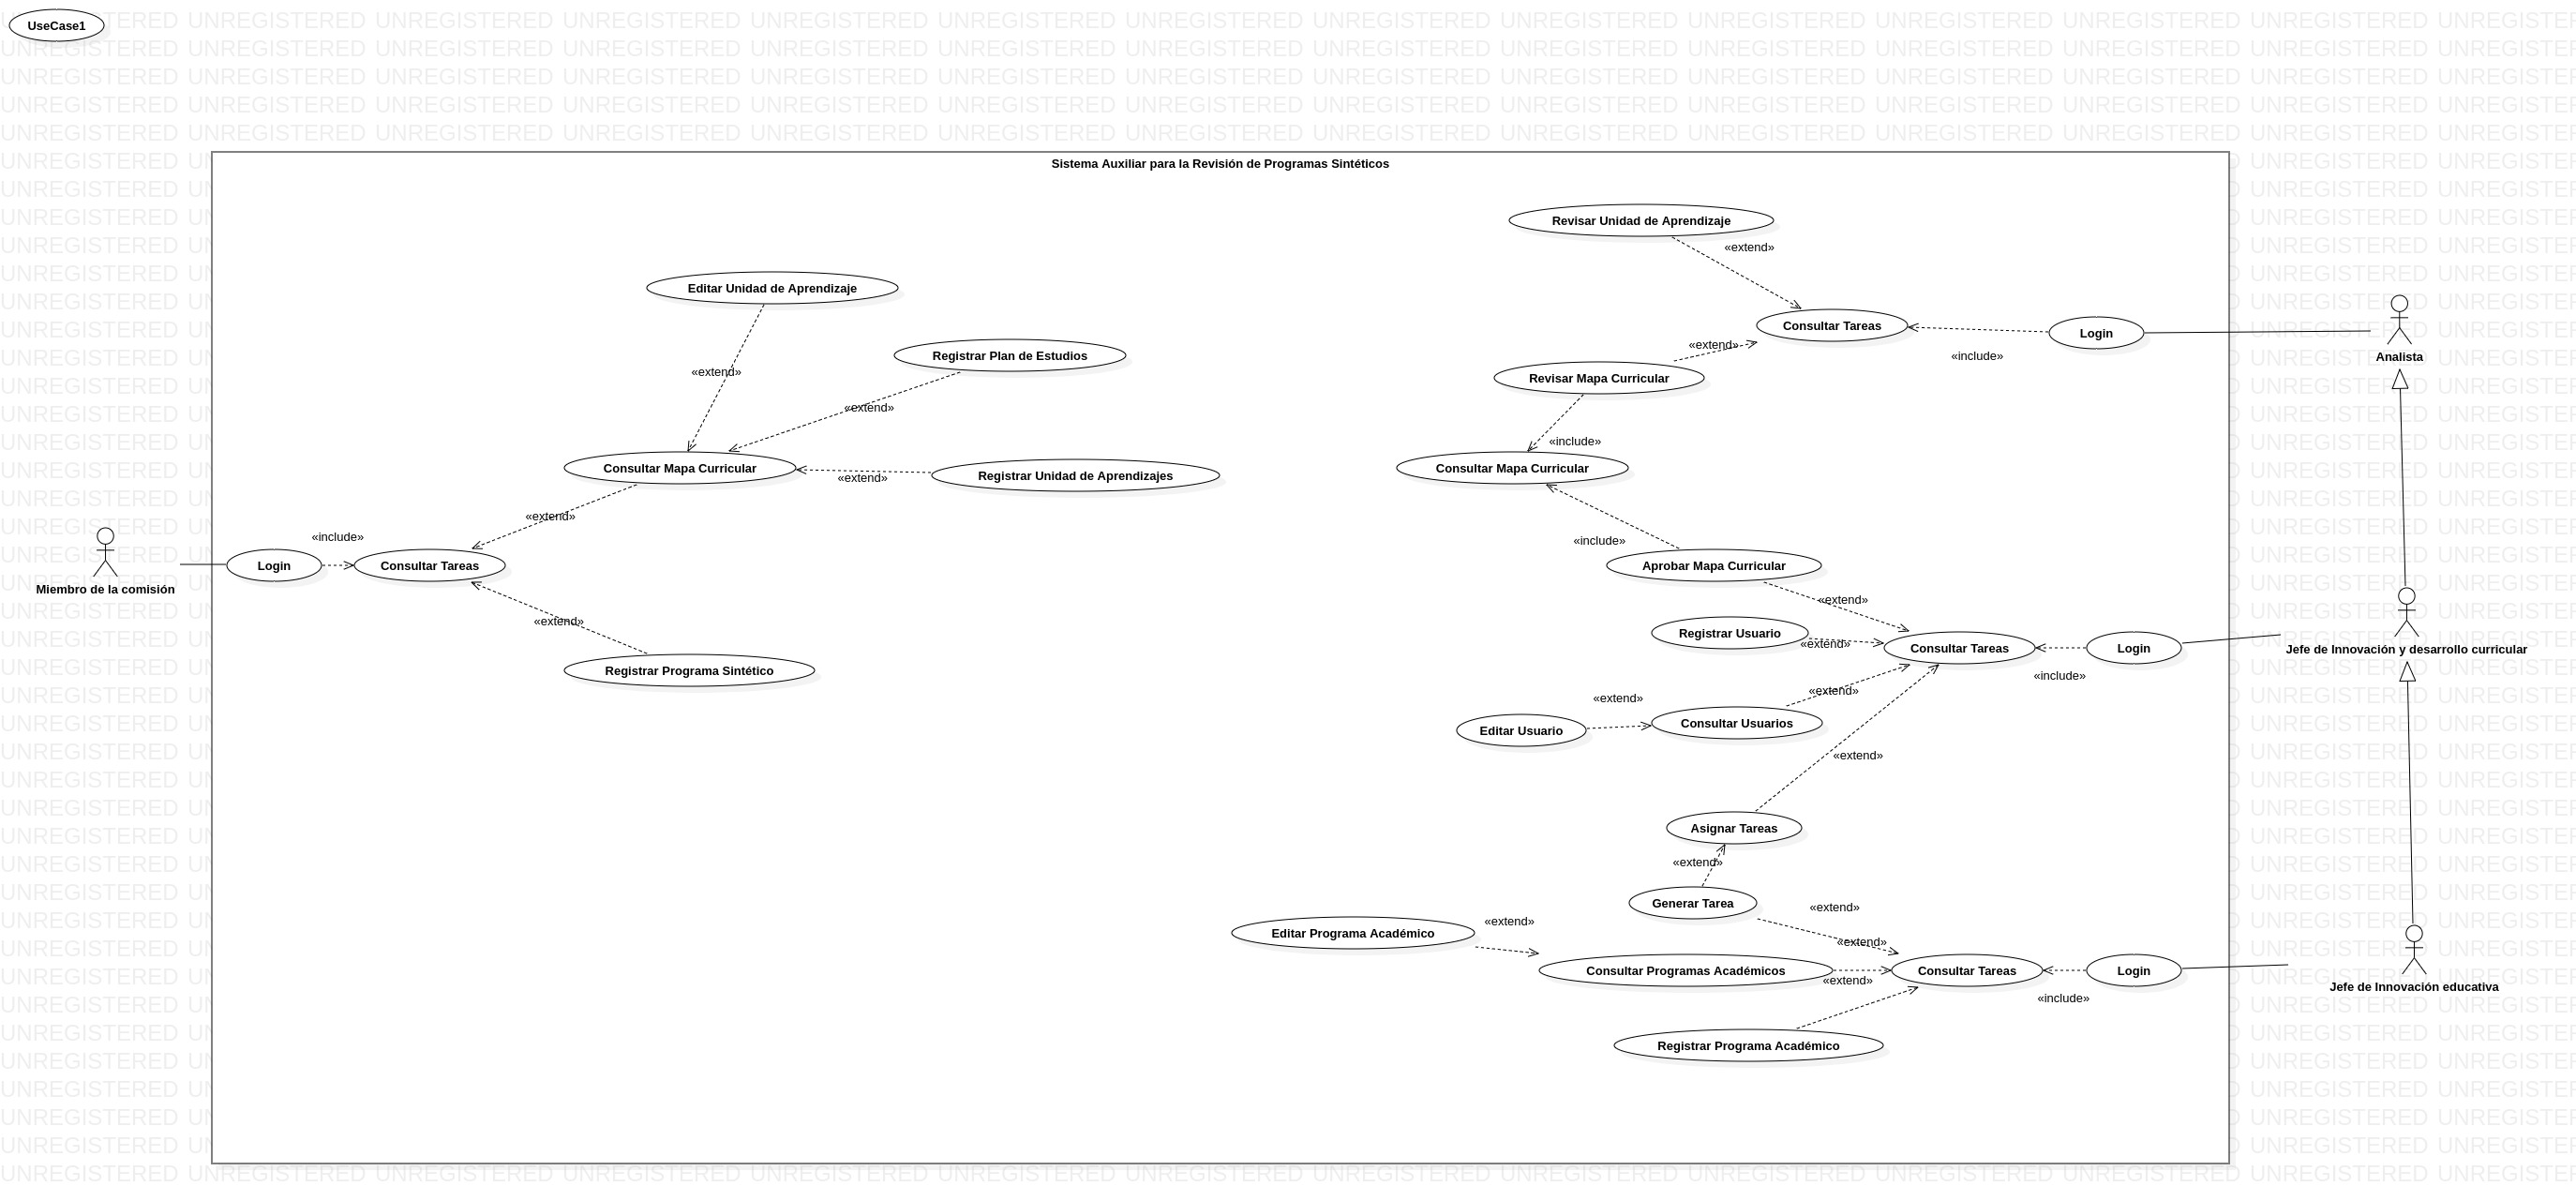
\includegraphics[width=.95\textwidth]{C2-DR/SP4/Image/CasosDeUso}
		\caption{Casos de Uso Subproceso para la  Carga del Mapa Curricular}
		\label{DCU-4}
	\end{center}
\end{figure}

\begin{center}
	\begin{tabular}{|c|c|c|c|}
		\hline
		ID        & Caso de uso                        & Requerimientos                                           & Encargado \\ \hline
        SP4-CU1   & Registrar Programa Académico       & \hyperref[SP4-U1]{SP4-U1}                                & Josué \\ \hline
        SP4-CU2   & Registrar Plan de Estudio          & \hyperref[SP4-U2]{SP4-U2}                                & Andrés \\ \hline
        SP4-CU3   & Registrar Unidad de Aprendizaje    & \hyperref[SP4-U3]{SP4-U3}                                & Andrés \\ \hline
        SP4-CU4   & Registrar Usuario                  & \hyperref[SP4-U4]{SP4-U4}                                & Arturo \\ \hline
        SP4-CU5   & Consultar Programas Académicos     & \hyperref[SP4-U5]{SP4-U5}                                & Josué \\ \hline
        SP4-CU6   & Consultar Mapa Curricular          & \hyperref[SP4-U8]{SP4-U8} y \hyperref[SP4-U6]{SP4-U6}    & Andrés \\ \hline
        SP4-CU7   & Consultar Usuarios                 & \hyperref[SP4-U7]{SP4-U7}                                & Arturo \\ \hline
        SP4-CU8   & Consultar Tareas                   & \hyperref[SP4-U9]{SP4-U9}                                & Arturo \\ \hline
        SP4-CU9   & Editar Programa Académico          & \hyperref[SP4-U21]{SP4-U21}                              & Josué \\ \hline
        SP4-CU10  & Editar Planes de Estudios          & \hyperref[SP4-U22]{SP4-U22}                              & Andrés \\ \hline
        SP4-CU11  & Editar Unidad de Aprendizaje       & \hyperref[SP4-U16]{SP4-U16}                              & Andrés \\ \hline
        SP4-CU12  & Editar Usuario                     & \hyperref[SP4-U23]{SP4-U23}                              & Josué \\ \hline
        SP4-CU13  & Aprobar Mapa Curricular            & \hyperref[SP4-U19]{SP4-U19}                              & Josué \\ \hline
        SP4-CU14  & Revisar Mapa Curricular            & \hyperref[SP4-U18]{SP4-U18}                              & Josué \\ \hline
        SP4-CU15  & Asignar Tarea                      & \hyperref[SP4-U11]{SP4-U11}                              & Arturo \\ \hline
        SP4-CU16  & Asignar Tareas                     & \hyperref[SP4-U11]{SP4-U11}                              & Arturo \\ \hline
        SP4-CU17  & Generar Tarea                      & \hyperref[SP4-U12]{SP4-U12}                              & Arturo \\ \hline
    \end{tabular}
\end{center}
\begin{UseCase}[marker]{SP4-CU1}{01}
  {
      Descripción larga e informal del Use Case
  }
  \UCitem{Version}{Version del Use Case}
  \UCitem{Super UC}{Use Case del que hereda}
  \UCitem{Propósito o Justificación}{Razón del use case del Use Case}
  \UCitem{Objetivo}{Objetivo final del Use Case}
  \UCitem{Precondiciones}{Estado inicial necesario para ejecutar el Use Case}
  \UCitem{Entradas}{Datos de entrada: Nombre, tipo y descripción}
  \UCitem{Salidas}{Datos de salida o resultados esperados}
  \UCitem{Resumen}{Se identifica al usuario por medio de su Login y Password}
  \UCitem{Postcondiciones}{Estado final del sistema después del Use Case}
  \UCitem{Restricciones}{Requerimientos no funcionales que debe cumplir}
  \UCitem{Suposiciones}{Hechos que se consideran reales para la descripción de este Use Case}
  \UCitem{Área}{Area o grupo a la que pertenece el Use Case}
  \UCitem{Referencias}{Documentos, personas o especificaciones que proporcionaron información para la especificación de este UseCase}Message
  \UCitem{Autor}{Nombre del responsable de la especificación del Use Case o de las modificaciones de la versión}
  \UCitem{Fecha}{Fecha de el último cambio al Use Case}

\end{UseCase}

% \UCEDdef{condición}{región}{casos de uso a los que extiende}
% \begin{UCtrayectoria}{prefijo}{nombre}
% 	\UCpaso[\UCActor] El actor oprime el boton buscar
% 	\UCpaso[\UCsist] El sistema ...
% \end{UCtrayectoria}
% \begin{UCtrayectoriaA}{Id}{Condicion}
% 	\UCpaso[\UCActor] El actor oprime el boton buscar
% 	\UCpaso[\UCsist] El sistema ...
% \end{UCtrayectoriaA}
% \input{C2-DR/SP4/Casos/SP4-CU1/RegistrarProgramaAcademico}
% \input{C2-DR/SP4/Casos/SP4-CU2/RegistrarPlanDeEstudio}
% \input{C2-DR/SP4/Casos/SP4-CU3/RegistrarUnidadDeAprendizaje}
% \input{C2-DR/SP4/Casos/SP4-CU4/RegistrarUsuario}
% \input{C2-DR/SP4/Casos/SP4-CU5/ConsultarProgramaAcademico}
% \input{C2-DR/SP4/Casos/SP4-CU6/ConsultarMapaCurricular}
% \input{C2-DR/SP4/Casos/SP4-CU7/ConsultarUsuarios}
% \input{C2-DR/SP4/Casos/SP4-CU8/ConsultarTareas}
% \input{C2-DR/SP4/Casos/SP4-CU9/EditarProgramaAcademico}
% \input{C2-DR/SP4/Casos/SP4-CU10/EditarPlanDeEstudio}
% \input{C2-DR/SP4/Casos/SP4-CU11/EditarUnidadDeAprendizaje}
% \input{C2-DR/SP4/Casos/SP4-CU12/EditarUsuario}
% \input{C2-DR/SP4/Casos/SP4-CU13/AprobarMapaCurricular}
% \input{C2-DR/SP4/Casos/SP4-CU14/RevisarMapaCurricular}
% \input{C2-DR/SP4/Casos/SP4-CU15/AsignarTareas}
% \input{C2-DR/SP4/Casos/SP4-CU16/AsignarTarea}
% \input{C2-DR/SP4/Casos/SP4-CU17/GenerarTarea}